\section{存储器层次结构}
\subsection{存储技术}
\subsubsection{随机访问存储器}

\paragraph{SRAM 和 DRAM}
\begin{itemize}
    \item \textbf{静态随机存取存储器}(SRAM, Static Random Access Memory):SRAM 将每个位存储在一个双稳态的 (bistable) 存储器单元里。每个单元由一个六晶体管电路实现。
    \item \textbf{动态随机存取存储器}(DRAM, Dynamic Random Access Memory):DRAM 的每个单元由一个电容和一个访问晶体管组成。它对干扰非常敏感,当电容的电压被扰乱之后,它就永远不会恢复了。
\end{itemize}

只要有供电,SRAM 就会保持不变。与 DRAM 不同,它不需要刷新。SRAM 的存取比 DRAM 快得多。SRAM 对诸如光和电噪声这样的干扰不敏感。代价是 SRAM 单元比 DRAM 单元使用更多的晶体管,因而密度低,而且更贵,功耗更大。
\begin{figure}[H]
    \centering
    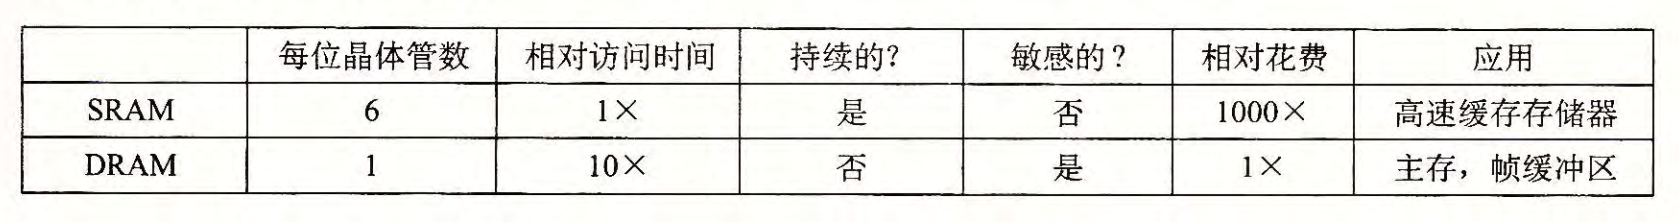
\includegraphics[width=0.8\textwidth]{memory/SRAM-DRAM.png}
\end{figure}

\paragraph{传统的 DRAM}

DRAM 芯片中的单元(位)被分成 d 个超单元 (supercell),每个超单元都由 w 个 DRAM
单元组成。 一个 d*w 的 DRAM 总共存储了 d*w 位信息。超单元被组织成一个 r 行 c 列的长
方形阵列,这里 r*c = d。每个超单元有形如 (i,j) 的地址,这里 i 表示行,而 j 表示列。

每个 DRAM 芯片被连接到某个称为内存控制器 (memory controller) 的电路,这个电
路可以一次传送 w 位到每个 DRAM 芯片或一次从每个 DRAM 芯片传出 w 位。为了读出
超单元 (i,j) 的内容,内存控制器将行地址 i 发送到 DRAM,然后是列地址 j。DRAM 把
超单元 (i,j) 的内容发回给控制器作为响应。行地址请求称为 RAS (Row Access Strobe, 行
访问选通脉冲),列地址请求称为 CAS (Column Access Strobe, 列访问选通脉冲)。注意,RAS
和 CAS 请求共享相同的 DRAM 地址引脚。

\begin{figure}[H]
    \centering
    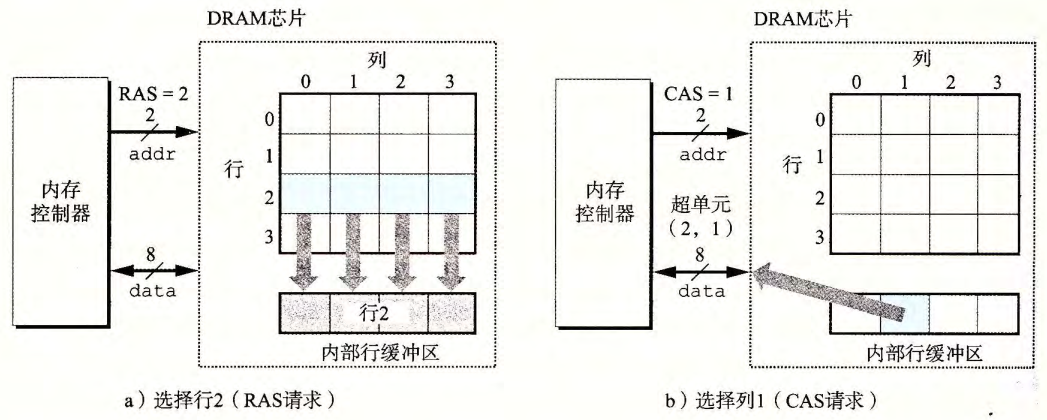
\includegraphics[width=0.8\textwidth]{memory/DRAM-read.png}
\end{figure}

\paragraph{内存模块}
DRAM 芯片封装在内存模块 (memory module) 中,插入到主板的扩展插槽上。
要取出内存地址 A 处的一个字,内存控制器将 A 转换成一个超单元地址 (i, j) 并将
它发送到内存模块,然后内存模块再将 i 和 j 广播到每个 DRAM 芯片。作为响应,每个
DRAM 输出它的 (i, j) 超单元的 8 位内容。模块中的电路收集这些输出,并把它们合并成
一个 64 位字,再返回给内存控制器。
\begin{figure}[H]
    \centering
    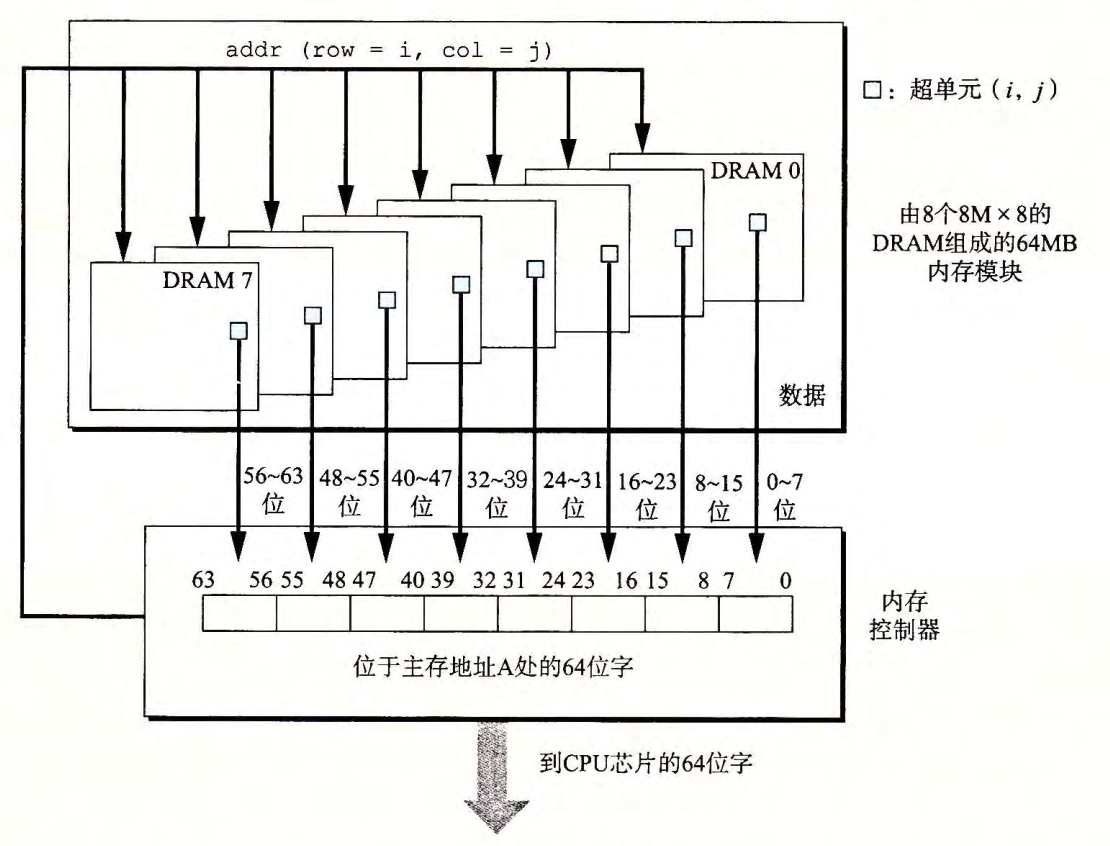
\includegraphics[width=0.8\textwidth]{memory/memory-module.png}
\end{figure}

\paragraph{增强的 DRAM}
\begin{itemize}
    \item 快页模式 DRAM (Fast Page Mode DRAM, FPM DRAM)
    \item 拓展数据输出 DRAM (Extended Data Out DRAM, EDO DRAM)
    \item 同步 DRAM (Synchronous DRAM, SDRAM)
    \item 双数据速率同步 DRAM (Double Data Rate Synchronous DRAM, DDR SDRAM)
    \item 视频 RAM (Video RAM, VRAM)
\end{itemize}

\paragraph{非易失性存储器}
如果断电, DRAM 和 SRAM 会丢失它们的信息,从这个意义上说,它们是易失的
(volatil) 。非易失性存储器 (nonvolatile memory) 即使是在关电后,仍然保存
着它们的信息。
\begin{itemize}
    \item 只读存储器 (Read-Only Memory, ROM)
    \item 可编程只读存储器 (Programmable Read-Only Memory, PROM)
    \item 可擦除可编程只读存储器 (Erasable Programmable Read-Only Memory, EPROM)
    \item 电可擦除可编程只读存储器 (Electrically Erasable Programmable Read-Only Memory, EEPROM)
    \item 闪存 (Flash Memory)
\end{itemize}

\paragraph{访问主存}
数据流通过称为总线 (bus) 的共享电子电路在处理器和 DRAM 主存之间来来回回。每
次 CPU 和主存之间的数据传送都是通过一系列步骤来完成的,这些步骤称为总线事务
(bus transaction) 。读事务 (read transaction) 从主存传送数据到 CPU 。写事务 (write transaction) 从 CPU 传送数据到主存。

下图的主要部件是 CPU 芯片、 I/O
桥接器 (I/O bridge) ,以及组成主存的 DRAM 内存模块。
这些部件由一对总线连接起来,其中一条总线是系统总线 (system bus) , 它连接 CPU 和
I/O 桥接器,另一条总线是内存总线 (memory bus), 它连接 I/O 桥接器和主存。 I/O 桥接
器将系统总线的电子信号翻译成内存总线的电子信号。 I/O 桥也将
系统总线和内存总线连接到 I/O 总线,像磁盘和图形卡这样的 I/O 设备共享 I/O 总线。

\begin{figure}[H]
    \centering
    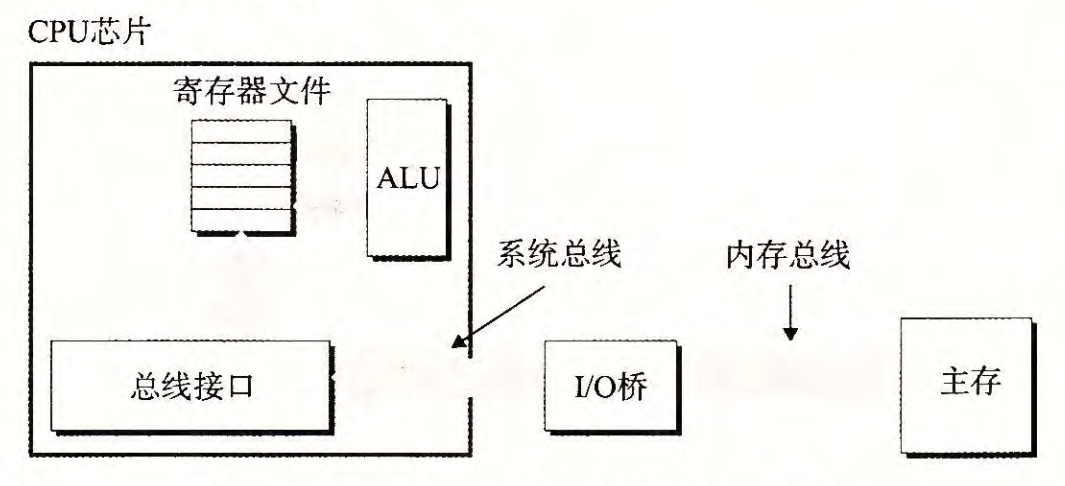
\includegraphics[width=0.8\textwidth]{memory/bus.png}
\end{figure}
\begin{figure}[H]
    \centering
    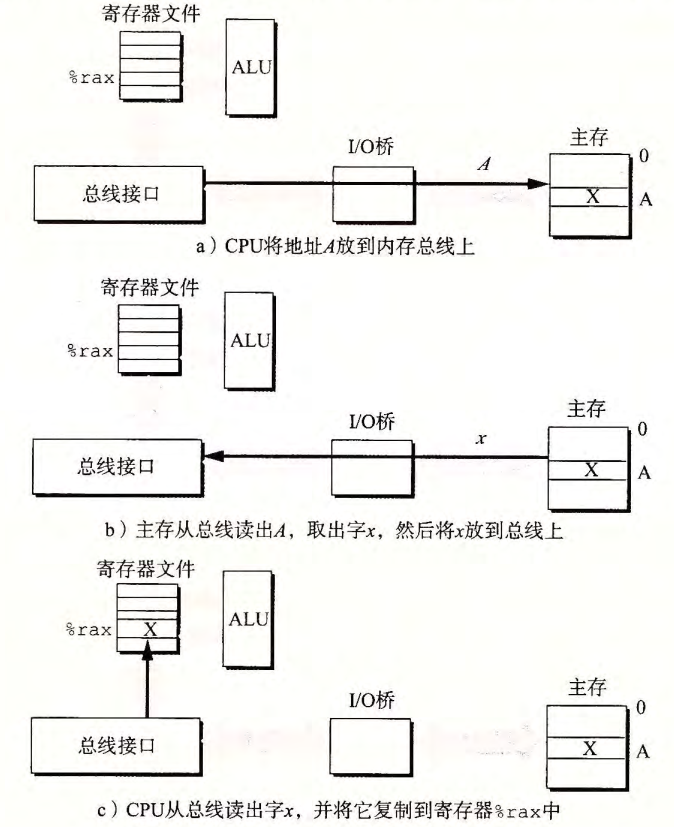
\includegraphics[width=0.8\textwidth]{memory/bus-transaction.png}
\end{figure}

\subsubsection{磁盘存储}
\paragraph{磁盘构造}
磁盘是由盘片 (platter) 构成的。每个盘片有两面,称为表面 (surface),表面覆盖着磁性记录材料。盘片中央有一个可以旋转的主轴 (spindle),它使得盘片以固定的旋转速率 (rotational rate) 旋转,通常是每分钟几千转 (revolutions per minute, RPM)。

每个表面是由一组称为磁道 (track) 的同心圆组成的。每个磁道被划分为一组扇区 (sector)。扇区之间由一些间隙 (gap) 分隔开,这些间隙中不存储数据位,间隙用于存放标识扇区的格式化信息。

磁盘是由一个或多个叠放在一起的盘片组成的,它们被封装在一个密封的包装里,整个装置通常被称为磁盘驱动器 (disk drive),我们通常简称为磁盘 (disk)。

\begin{figure}[H]
    \centering
    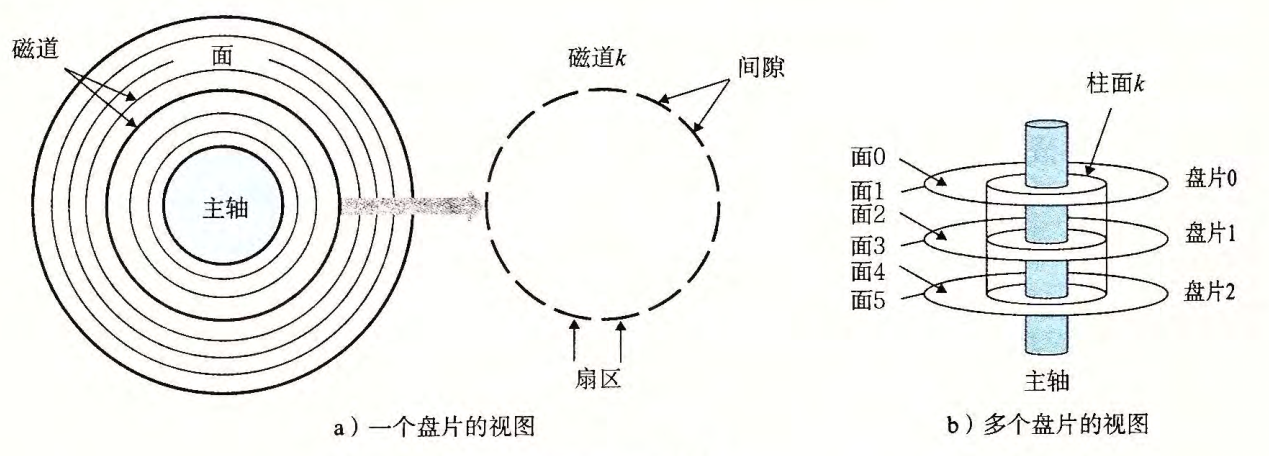
\includegraphics[width=0.8\textwidth]{memory/disk.png}
\end{figure}

\paragraph{磁盘容量}
\begin{itemize}
    \item 记录密度 (recording density):每英寸磁道上的位数。
    \item 轨道密度 (track density):每英寸径向轨道的数量。
    \item 面密度 (areal density):每平方英寸上的位数,记录密度和轨道密度的乘积。
\end{itemize}
\begin{center}
    磁盘容量 = 字节数/扇区 $\times$ 平均扇区数/磁道 $\times$ 磁道数/表面 $\times$ 表面数/盘片 $\times$ 盘片数/磁盘
\end{center}
\begin{sidenote}{-千兆字节有多大}
    对于与 DRAM 和 SRAM 容量相关的计量单位,通常 $K=2^{10}$,$M=2^{20}$,$G=2^{30}$ 而
    $T= 2^{40}$。对于与像磁盘和网络这样的 I/O 设备容量相关的计量单位,通常 $K = 10^{3}$,
    $M= 10^{6}$,$G = 10^{9}$,而 $T=10^{12}$。
\end{sidenote}

\paragraph{磁盘操作}

磁盘用读写头 (read/write head) 来读写存储在磁性表面的位,而读写头连接到一个传动臂 (actuator arm) 一端,
通过沿着半径轴前后移动这个传动臂,驱动器可以将读写头定位在盘面上的任何磁道上。
这样的机械运动称为寻道 (seek)。一旦读写头定位到了期望的磁道上,那么当磁道上的每个位通过它的下面时,
读写头可以感知到这个位的值(读该位),也可以修改这个位的值(写该位)。
有多个盘片的磁盘针对每个盘面都有一个独立的读写头。
读写头垂直排列,一致行动。在任何时刻,所有的读写头都位于同一个柱面上。

\begin{figure}[H]
    \centering
    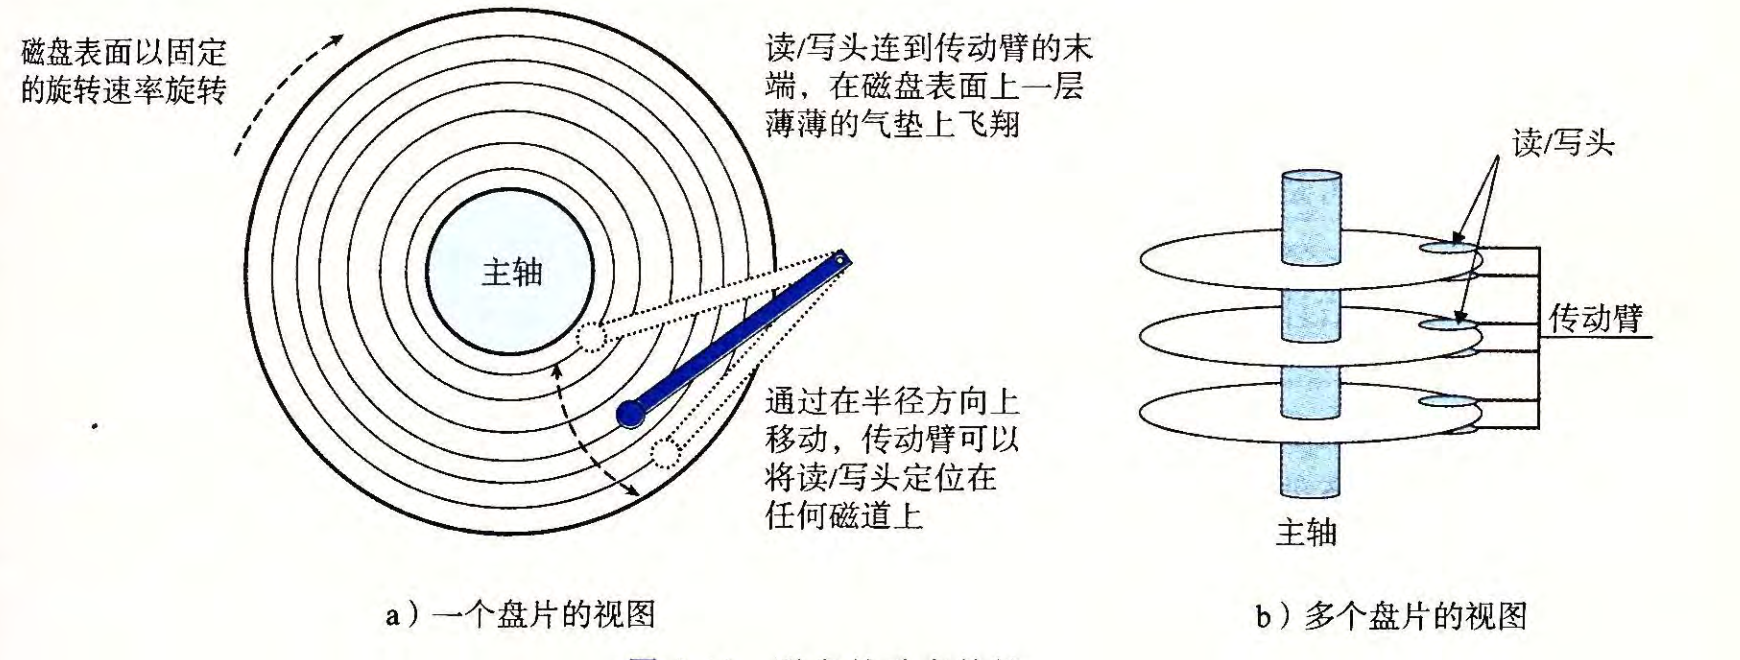
\includegraphics[width=0.8\textwidth]{memory/disk-operation.png}
\end{figure}

对扇区的访问时间 (access time) 有三个主要的部分:
\begin{itemize}
    \item 寻道时间 (seek time):将读/写头移动到正确磁道所需的时间。
    \item 延迟时间 (latency time):等待所需扇区旋转
    \item 传输时间 (transfer time):读写扇区所需的时间。
\end{itemize}

因为寻道时间和旋转延迟大致相等,所以将寻道时间乘 2 是估计磁盘访问时间的简单而合理的方法。

\paragraph{磁盘逻辑块}

磁盘封装中有一个小的硬件/固件设备,称为磁盘控制器,维护着逻辑块号和实际(物理)磁盘扇区之间的映射关系。

\paragraph{连接 I/O 设备}

例如图形卡、监视器、鼠标、键盘和磁盘这样的输入/输出 (I/O) 设备,都是通过 I/O
总线连接到
CPU 和主存的。

虽然 I/O 总线比系统总线和内存总线慢,但是它可以容纳种类繁多的第三方 I/O 设备:
\begin{itemize}
    \item 通用串行总线 (Universal Serial Bus, USB) 控制器
    \item 图形卡(或适配器)(Graphics Card/Adapter)
    \item 主机总线适配器 (Host Bus Adapter, HBA)
    \item 网络适配器 (Network Adapter)
\end{itemize}

\begin{figure}[H]
    \centering
    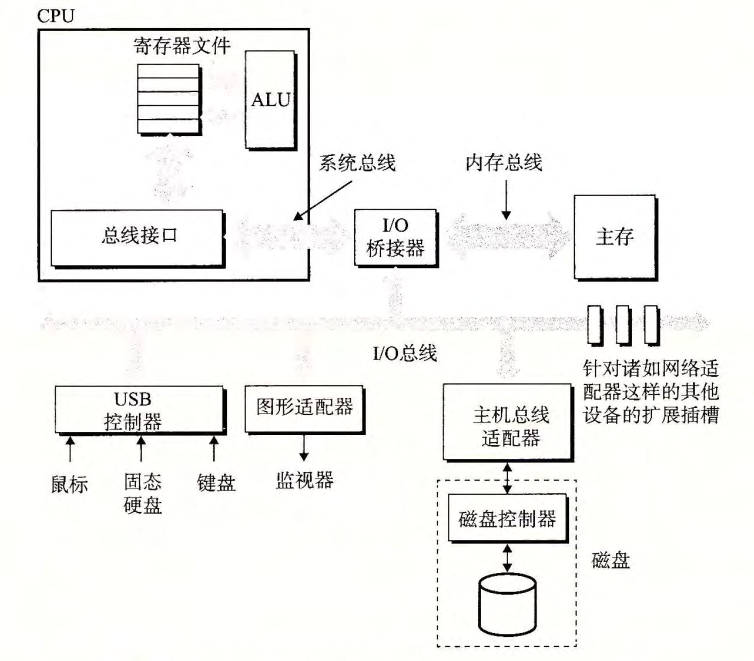
\includegraphics[width=0.8\textwidth]{memory/buses.png}
\end{figure}

\paragraph{访问磁盘}

\begin{figure}[H]
    \centering
    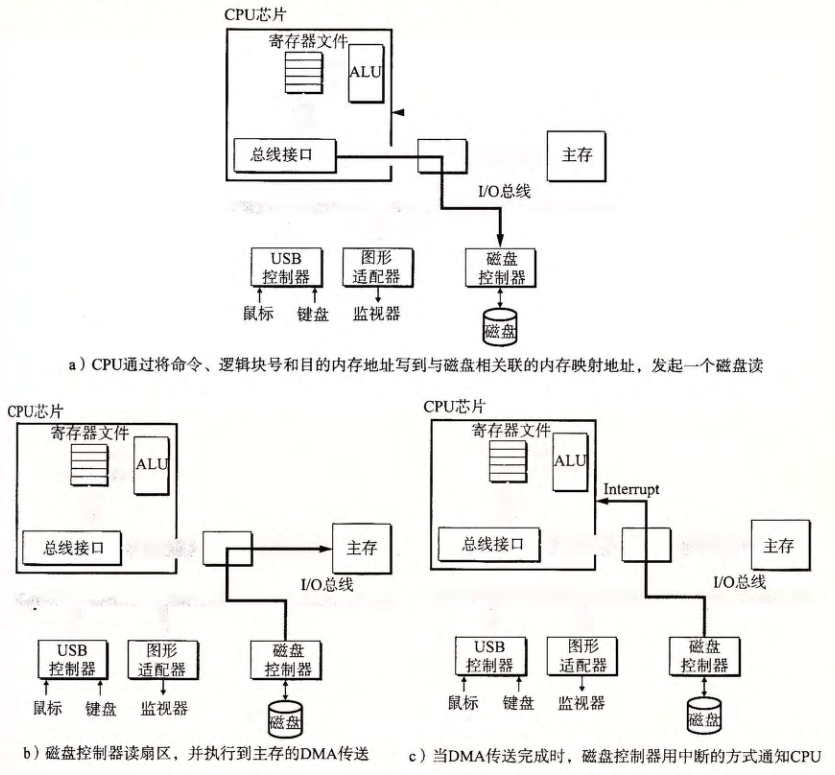
\includegraphics[width=0.8\textwidth]{memory/disk-access.png}
\end{figure}

\subsubsection{固态硬盘}

固态硬盘 (Solid State Disk, SSD) 是一种基于闪存的存储技术。一个 SSD 封装由一个或多个闪存芯片和闪存翻
译层 (flash translation layer) 组成,闪存芯片替代传统旋转磁盘中的机械驱动器,而闪存
翻译层是一个硬件/固件设备,扮演与磁盘控制器相同的角色,将对逻辑块的请求翻译成
对底层物理设备的访问。

\begin{figure}[H]
    \centering
    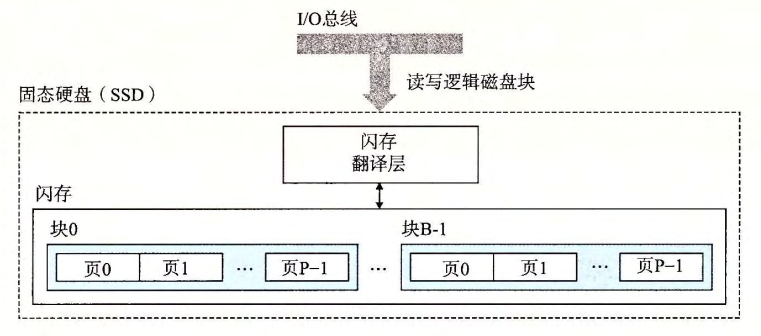
\includegraphics[width=0.8\textwidth]{memory/SSD.png}
\end{figure}

一个闪存由 B 个块的序列组成,每个块由 P 页组成。
数据是以页为单位读写的。
只有在一页所属的块整个被擦除之后,才能写这一页(通常是指该块中的所有位都被设置为 1)。
不过,一旦一个块被擦除了,块中每一个页都可以不需要再进行擦除就写一次。

\begin{sidenote}{局部性原理}
    局部性原理(Locality Principle)是计算机科学中的一个重要概念,指的是在程序执行过程中,访问的数据和指令往往集中在某些特定的区域。这种现象可以分为两种类型:时间局部性和空间局部性。

    \textbf{时间局部性}(Temporal Locality)指的是如果一个数据项在某个时间点被访问,那么在不久的将来它很可能会再次被访问。换句话说,最近使用过的数据很可能会再次被使用。

    \textbf{空间局部性}(Spatial Locality)指的是如果一个数据项在某个时间点被访问,那么与它相邻的数据项也很可能会在不久的将来被访问。换句话说,程序倾向于访问存储器中相近的地址。

    局部性原理是设计高效存储器层次结构(如缓存、主存和辅助存储器)的基础。通过利用局部性原理,计算机系统可以显著提高数据访问速度,减少延迟,从而提升整体性能。
\end{sidenote}


\subsection{缓存}
\subsubsection{存储器层次结构}

\begin{figure}[H]
    \centering
    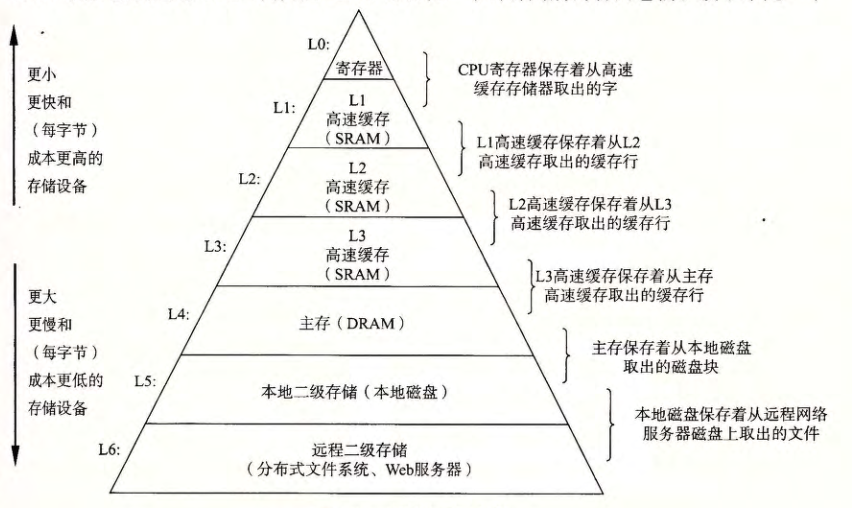
\includegraphics[width=0.8\textwidth]{memory/memory-hierarchy.png}
\end{figure}

\subsubsection{存储器层次结构中的缓存}

一般而言,高速缓存 (cache) 是一个小而快速的存储设备,它作为存储在更大、也更慢的设备中的数据对象的缓冲区域。
存储器层次结构的中心思想是,对于每个 k,位于 k 层的更快更小的存储设备作为位于 k+1 层的更大更慢的存储设备的缓存。

\begin{itemize}
    \item \textbf{缓存命中}(cache hit):当处理器请求的数据已经存在于缓存中时,就发生了缓存命中。
    \item \textbf{缓存未命中}(cache miss):当处理器请求的数据不在缓存中时,就发生了缓存未命中。
          \begin{itemize}
              \item \textbf{冷未命中}(cold miss):也称为初始未命中 (compulsory miss),当数据第一次被访问时发生,因为它还没有被加载到缓存中。
              \item \textbf{容量未命中}(capacity miss):当缓存的容量不足以容纳工作集 (working set) 时发生,即使缓存使用了最优的替换策略,也会发生这种未命中。
              \item \textbf{冲突未命中}(conflict miss):当多个数据块映射到缓存中的同一位置时发生,即使缓存有足够的容量,也会发生这种未命中。
              \item \textbf{一致性未命中}(coherence miss):在多处理器系统中,当一个处理器修改了缓存中的数据,而另一个处理器试图访问该数据时发生。
          \end{itemize}
\end{itemize}

\subsection{高速缓存存储器}
\subsubsection{通用的高速缓存存储器组织结构}

考虑一个计算机系统,其中每个存储器地址有 $m$ 位,形成 $M=2^m$ 个不同的地址。
一个机器的高速缓存被组织成一个有 $S=2^s$ 个高速缓存组 (cache set) 的数组。
每个组包含 $E$ 个高速缓存行 (cache line)。
每个行是由一个 $B=2^b$ 字节的数据块 (block) 组成的,一个有效位 (valid bit) 指明这个行是否包含有意义的信息,还有 $t=m-(h+s)$ 个标记位 (tag bit),它们唯一地标识存储在这个高速缓存行中的块。

\begin{figure}[H]
    \centering
    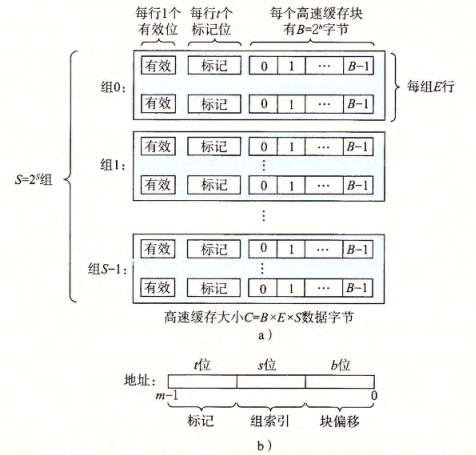
\includegraphics[width=0.8\textwidth]{memory/cache-organization.png}
\end{figure}

一般而言,高速缓存的结构可以用元组 ($C_S$, $E$, $B$, $m$) 来描述。高速缓存的大小(或
容量)$C$ 指的是所有块的大小的和。标记位和有效位不包括在内。因此,$C=S \times E \times B$。

\subsubsection{直接映射高速缓存}
根据每个组的高速缓存行数 $E$,高速缓存被分为不同的类。
每个组只有一行 ($E=1$) 的高速缓存称为直接映射高速缓存 (direct-mapped cache)。

\begin{figure}[H]
    \centering
    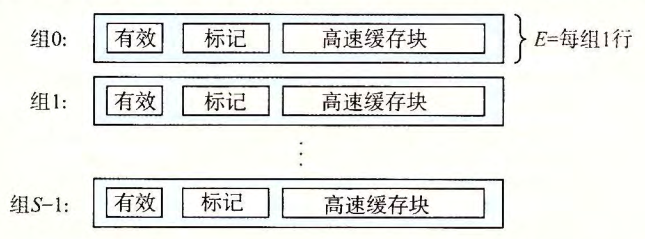
\includegraphics[width=0.8\textwidth]{memory/direct-mapped-cache.png}
\end{figure}

高速缓存确定一个请求是否命中,然后抽取出被请求的字的过程,分为三步:组选择;行匹配;字抽取。

\paragraph{直接映射高速缓存中的组选择}
高速缓存从 $w$ 的地址中间抽取出 $s$ 个组索引位。这些位被解释成一个对应于一个组号的无符号整数。
\begin{figure}[H]
    \centering
    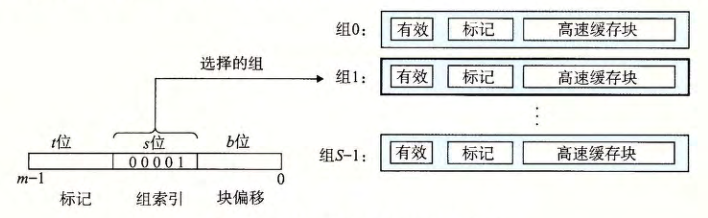
\includegraphics[width=0.8\textwidth]{memory/find-set.png}
\end{figure}

\paragraph{直接映射高速缓存中的行匹配}
确定是否有字 $w$ 的一个副本存储在组 $i$ 包含的一个高速缓存行中。
当且仅当设置了有效位,而且高速缓存行中的标记与 $w$ 的地址中的
标记相匹配时,这一行中包含 $w$ 的一个副本。
\begin{figure}[H]
    \centering
    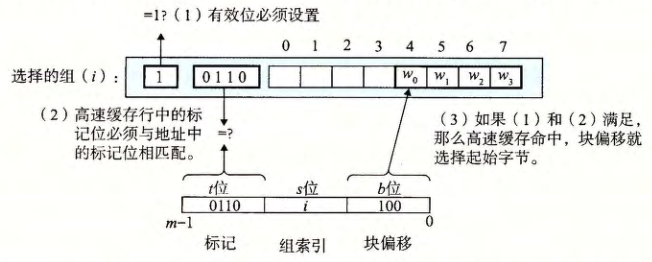
\includegraphics[width=0.8\textwidth]{memory/match-select.png}
\end{figure}

\paragraph{直接映射高速缓存中的字选择}
一旦命中,我们知道 $w$ 就在这个块中的某个地方。最后一步确定所需要的字在块中是
从哪里开始的。块偏移位提供了所需要的字的第一个字节的偏移。

\paragraph{直接映射高速缓存中不命中时的行替换}
如果缓存不命中,那么它需要从存储器层次结构中的下一层取出被请求的块,然后将
新的块存储在组索引位指示的组中的一个高速缓存行中。一般而言,如果组中都是有效高速
缓存行了,那么必须要驱逐出一个现存的行。对于直接映射高速缓存来说,每个组只包含有一行,替换策略非常简单:用新取出的行替换当前的行。

\begin{sidenote}{为什么用中间的位来索引}
    如果高位用做索引,那么一些连续的内存块就会映射到相同的高速缓存块。
    例如,在图中,头四个块映射到第一个高速缓存组,第二个四个块映射到第二个组,依此类推。
    如果一个程序有良好的空间局部性,顺序扫描一个数组的元素,那么在任何时刻,高速缓存都只保存着一个块大小的数组内容。
    这样对高速缓存的使用效率很低。
    相比较而言,以中间位作为索引,相邻的块总是映射到不同的高速缓存行。
    \begin{figure}[H]
        \centering
        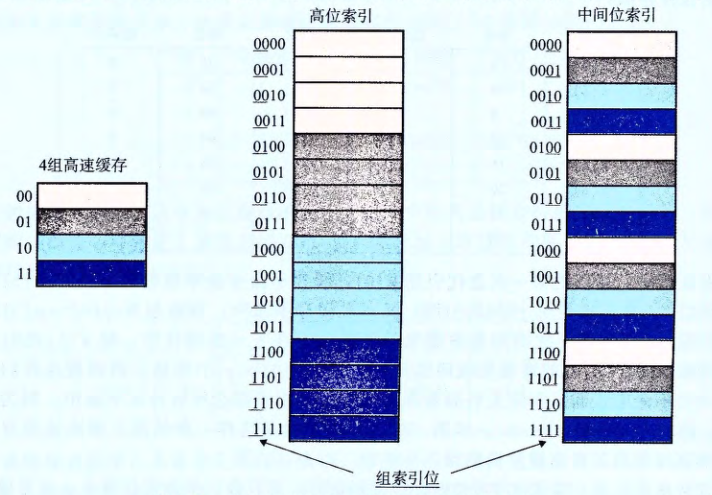
\includegraphics[width=0.8\textwidth]{memory/middle-bit-indexing.png}
    \end{figure}
\end{sidenote}

\subsubsection{组相联高速缓存}
直接映射高速缓存中冲突不命中造成的问题源千每个组只有一行(或者,按照我们的术语来描述就是 E=1 )这个限制。
组相联高速缓存 (set associative cache) 放松了这条限制,
所以每个组都保存有多个高速缓存行,通常称为 E 路组相联高速缓存。
\begin{figure}[H]
    \centering
    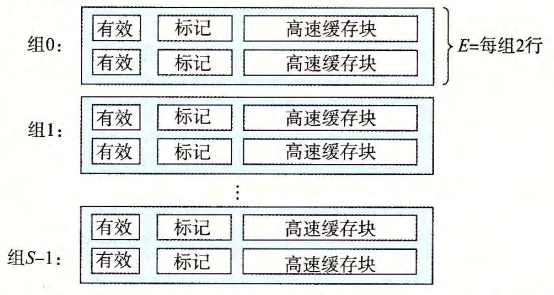
\includegraphics[width=0.8\textwidth]{memory/E-way-cache.png}
\end{figure}

\paragraph{组相联高速缓存中的组选择}
组选择与直接映射高速缓存的组选择一样,组索引位标识组。
\begin{figure}[H]
    \centering
    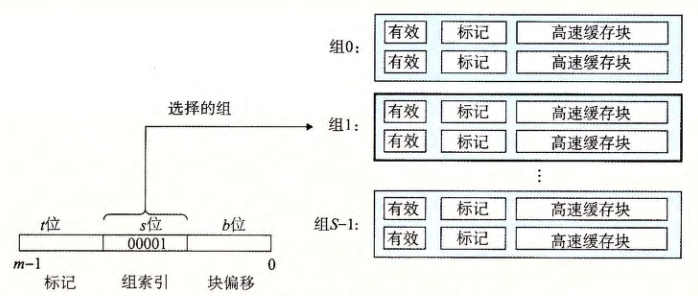
\includegraphics[width=0.8\textwidth]{memory/E-find-set.png}
\end{figure}

\paragraph{组相联高速缓存中的行匹配和字选择}
组相联高速缓存中的行匹配比直接映射高速缓存中的更复杂。高速缓存必须搜索组中的每一行,
寻找一个有效的行,其标记与地址中的标记相匹配 。如果高速缓存找到了这样一行,那么
我们就命中,块偏移从这个块中选择一个字。
\begin{figure}[H]
    \centering
    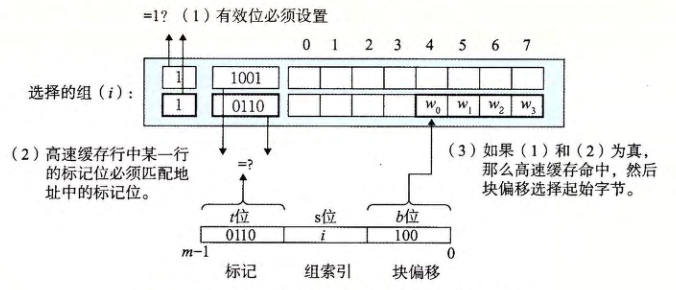
\includegraphics[width=0.8\textwidth]{memory/E-match-select.png}
\end{figure}

\paragraph{组相联高速缓存中不命中时的行替换}
如果 CPU 请求的字不在组的任何一行中,那么就是缓存不命中,高速缓存必须从内
存中取出包含这个字的块。不过,一旦高速缓存取出了这个块,该替换哪个行呢?当然,
如果有一个空行,那它就是个很好的候选。但是如果该组中没有空行,那么我们必须从中
选择一个非空的行,希望 CPU 不会很快引用这个被替换的行。

最简单的替换策略是随机选择要替换的行。其他更复杂的策略利用了局部性原理,以使在比较近的将来引用被替换的行的概率最小。
例如,最不常使用 (Least-Frequently-Used, LFU) 策略会替换在过去某个时间窗口内引用次数最少的那一行。
最近最少使用 (LeastRecently-Used, LRU) 策略会替换最后一次访问时间最久远的那一行。

\subsubsection{全相联高速缓存}
全相联高速缓存 (fully associative cache) 是由一个包含所有高速缓存行的组组成的高速缓存。
\begin{figure}[H]
    \centering
    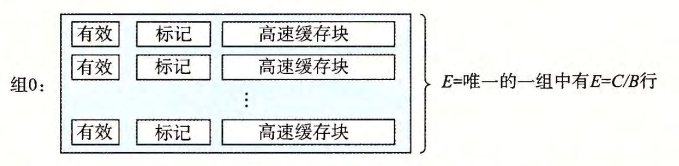
\includegraphics[width=0.8\textwidth]{memory/fully-associative-cache.png}
\end{figure}

\paragraph{全相联高速缓存中的组选择}
注意,全相联高速缓存地址中没有组索引位,地址只被划分成了一个标记和一个块偏移,因为只有一个组。
\begin{figure}[H]
    \centering
    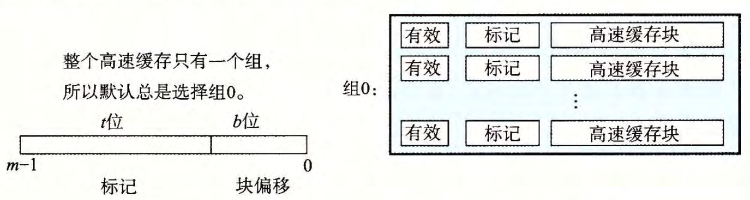
\includegraphics[width=0.8\textwidth]{memory/fully-find-set.png}
\end{figure}

\paragraph{全相联高速缓存中的行匹配和字选择}
全相联高速缓存中的行匹配和字选择与组相联高速缓存中的是一样的,它们之间的区别主要是规模大小的问题。
\begin{figure}[H]
    \centering
    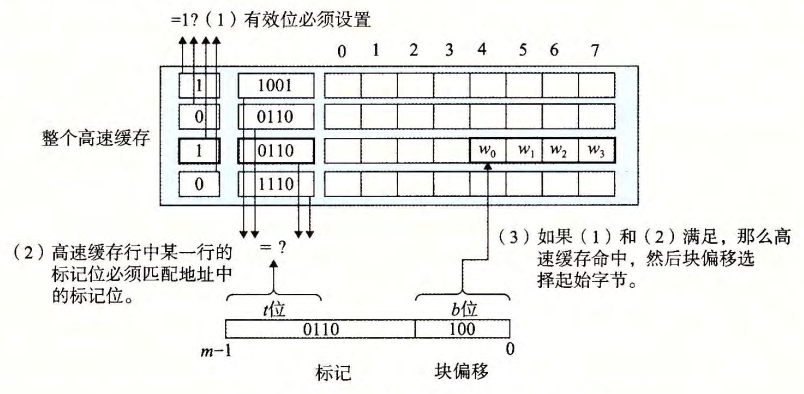
\includegraphics[width=0.8\textwidth]{memory/fully-match-select.png}
\end{figure}

因为高速缓存电路必须并行地搜索许多相匹配的标记,构造一个又大又快的相联高速缓存很困难,而且很昂贵。
因此,全相联高速缓存只适合做小的高速缓存。

\subsubsection{高速缓存的写操作}
假设我们要写一个已经缓存了的字 w (write hit)。

最简单的方法,称为直写 (write-through),就是立即将 w 的高速缓存块写回到紧接着
的低一层中。虽然简单,但是直写的缺点是每次写都会引起总线流量。

另一种方法,称为写回 (write-back),尽可能地推迟更新,只有当替换算法要驱逐这个更新过的块时,才把
它写到紧接着的低一层中。由于局部性,写回能显著地减少总线流量,但是它的缺点是增
加了复杂性。高速缓存必须为每个高速缓存行维护一个额外的修改位 (dirty bit),表明这个高速缓存块是否被修改过。

另一个问题是如何处理写不命中。

一种方法,称为写分配 (write-allocate),加载相应
的低一层中的块到高速缓存中,然后更新这个高速缓存块。写分配试图利用写的空间局部
性,但是缺点是每次不命中都会导致一个块从低一层传送到高速缓存。

另一种方法,称为非写分配 (not-write-allocate),避开高速缓存,直接把这个字写到低一层中。

直写高速缓存通常是非写分配的。写回高速缓存通常是写分配的。

\subsubsection{高速缓存参数的性能影响}
有许多指标来衡量高速缓存的性能:
\begin{itemize}
    \item \textbf{命中率}(hit rate):命中次数与总访问次数之比。
    \item \textbf{未命中率}(miss rate):未命中次数与总访问次数之比,未命中率 = 1 - 命中率。
    \item \textbf{命中时间}(hit time):从高速缓存传送一个字到 CPU 所需的时间,包括组选择、行确认和字选择的时间。
    \item \textbf{未命中惩罚}(miss penalty):由未命中所需要的额外的时间。从低一层存储器传送一个块到高速缓存所需的时间,包括传输时间和处理未命中的时间。
\end{itemize}

优化高速缓存的成本和性能的折中是一项很精细的工作,但也有一些定性的折中考量:
\begin{itemize}
    \item 高速缓存大小:增大高速缓存的大小通常会提高命中率,但可能会增加命中时间。
    \item 块大小:增大块大小可以利用空间局部性,帮助提高命中率,但可能会增加未命中惩罚。
          对于给定的高速缓存大小,块越大就意味着高速缓存行数越少,这会损害时间局部性比空间局部性更好的程序中的命中率。
    \item 组相联度:增大组相联度通常会降低高速缓存由于冲突不命中出现抖动的可能性。不过,较高的相联度会造成较高的成本。
          较高的相联度会增加命中时间,因为复杂性增加了,另外,还会增加不命中处罚,因为选择牺牲行的复杂性也增加了。
    \item 写策略:写回通常比直写更复杂,但它能显著地减少总线流量,从而降低未命中惩罚。
\end{itemize}

\subsection{高速缓存友好的代码}
确保代码高速缓存友好有一些基本方法:
\begin{itemize}
    \item 让最常见的情况运行得快。把注意力集中在核心函数里的循环上,而忽略其他部分。
    \item 尽量减小每个循环内部的缓存不命中数量。
\end{itemize}
\subsubsection{存储器山}
\begin{figure}[H]
    \centering
    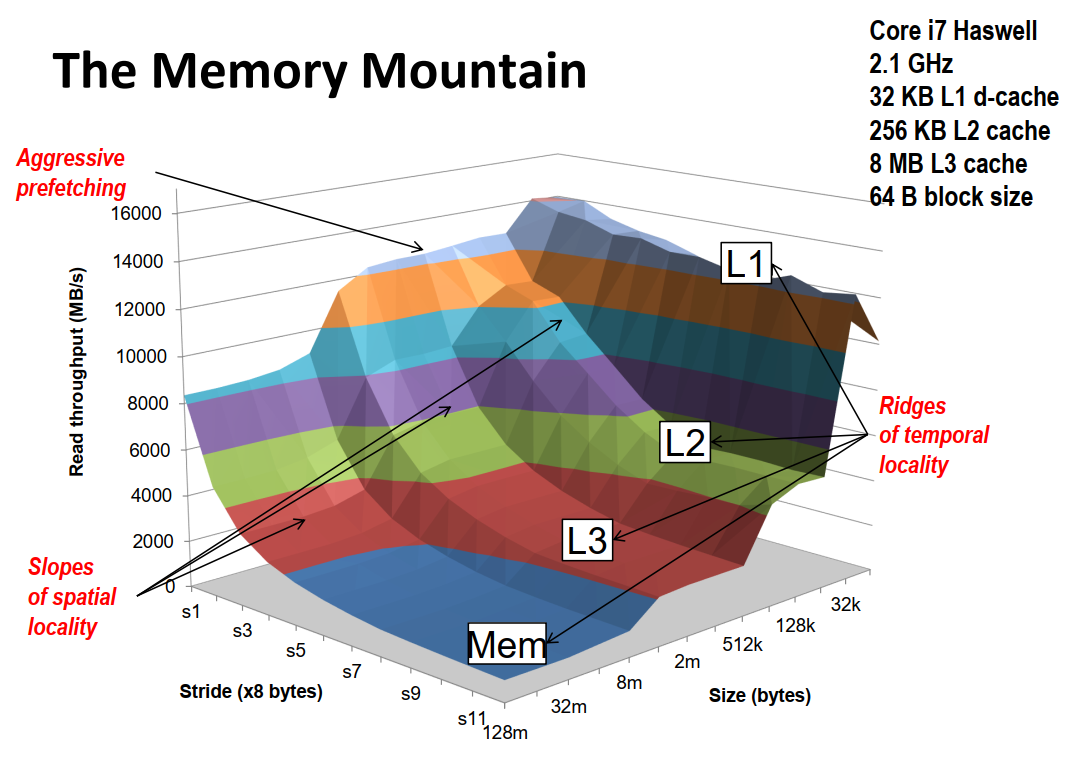
\includegraphics[width=0.8\textwidth]{memory/memory-mountain.png}
\end{figure}

\subsubsection{一维数组}
一般而言,如果一个高速缓存的块大小为 B 字节,那么一个步长为 k 的引用模式(这里 k 是
以字为单位的)平均每次循环迭代会有 min(1, (wordsize*k)/B) 次缓存不命中。
所以步长为 1 的引用确实是高速缓存友好的。
\subsubsection{二维数组}
行优先顺序:等同于步长为 1 的访问模式。

列优先顺序:如果足够幸运,整个数组都在高速缓存中,那么也会同行优先一样。如果数组比高速缓存要大,那么每次对 a[i][j] 的访问都会不命中!

\subsubsection{矩阵乘法}
矩阵乘法函数通常是用 3 个嵌套的循环来实现的,分别用索引 i、j 和 k 来标识。如果改变
循环的次序,对代码进行一些其他的小改动,我们就能得到矩阵乘法的 6 个在功能上等价
的版本。为了分析,我们做如下假设:
\begin{itemize}
    \item 每个数组都是一个 double 类型的 n*n 的数组。
    \item 只有一个高速缓存,其块大小为 32 字节 (B=32)。
    \item 数组大小 n 很大,以至于矩阵的一行都不能完全装进 L1 高速缓存中。
    \item 编译器将局部变量存储到寄存器中,因此循环内对局部变量的引用不需要任何加载或存储指令。
\end{itemize}
\begin{figure}[H]
    \centering
    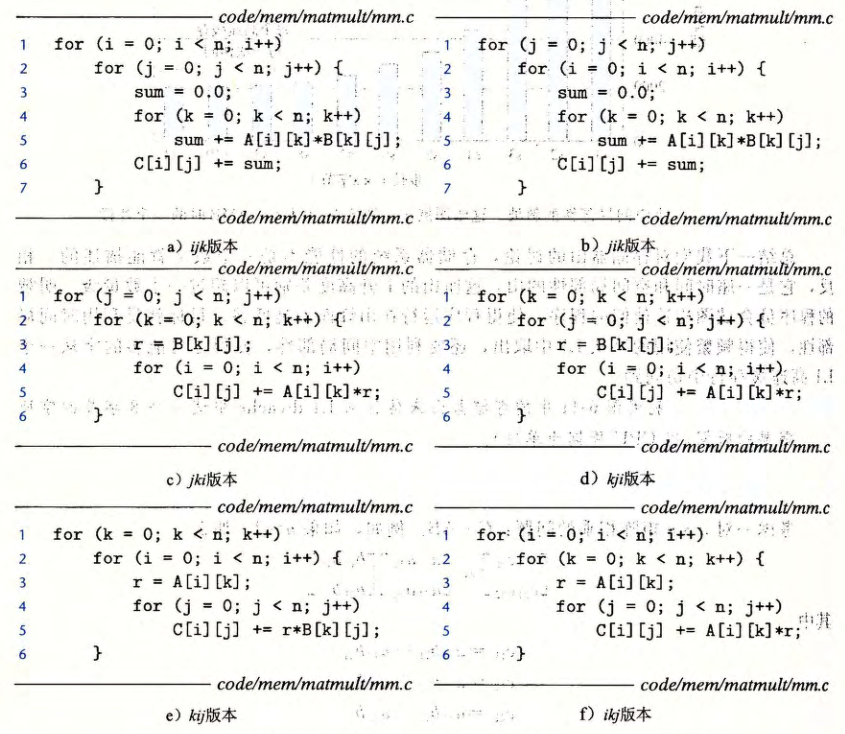
\includegraphics[width=0.8\textwidth]{memory/matrix-multiplication.png}
\end{figure}

类 AB 例程的内循环以步长 1 扫描数组 A 的行。
因为每个高速缓存块保存四个 8 字节的字,A 的不命中率是每次迭代不命中 0.25 次。
另一方面,内循环以步长 n 扫描数组B 的一列。
因为 n 很大,每次对数组 B 的访问都会不命中,所以每次迭代总共会有 1.25 次不命中。

类 AC 例程的内循环每次迭代执行两个加载和一个
存储(相对类 AB 例程,它们执行 2 个加载而没有存储)。内循环以步长 n 扫描 A 和 C 的
列。结果是每次加载都会不命中,所以每次迭代总共有两个不命中。

BC 例程使用了两个加载和一个存储,它们比 AB 例程多需要一个内存操作。
内循环以步长为 1 的访问模式按行扫描 B 和 C,每次迭代每个数组上的不命中率只有 0.25 次不命中,
所以每次迭代总共有 0.75 个不命中。

\begin{figure}[H]
    \centering
    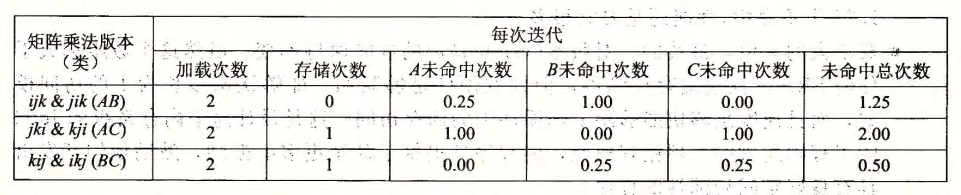
\includegraphics[width=0.8\textwidth]{memory/matrix-multiplication-analysis.png}
\end{figure}

\subsubsection{分块}
分块的大致思想是将一个程序中的数据结构组织成的大的片,称为块 (block)。
这样构造程序,使得能够将一个片加载到 L1 高速缓存中,并在这个片中进行所需的所有的读和写,
然后丢掉这个片,加载下一个片,依此类推。

与为提高空间局部性所做的简单循环变换不同,分块使得代码更难阅读和理解。
由于这个原因,它最适合于优化编译器或者频繁执行的库函数。

假设:
\begin{itemize}
    \item 数组都一个 double 类型的 n*n 的数组。
    \item block = 8 doubles * 8 doubles。
    \item 缓存容量 C 远小于 n。
\end{itemize}

若不采用分块策略:
\begin{figure}[H]
    \centering
    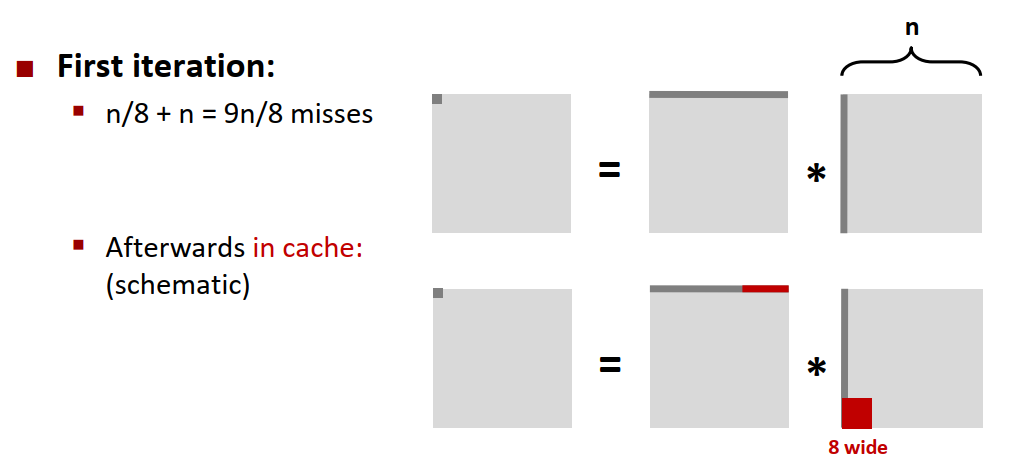
\includegraphics[width=0.8\textwidth]{memory/matrix-multiplication-unblocked-1.png}
\end{figure}
\begin{figure}[H]
    \centering
    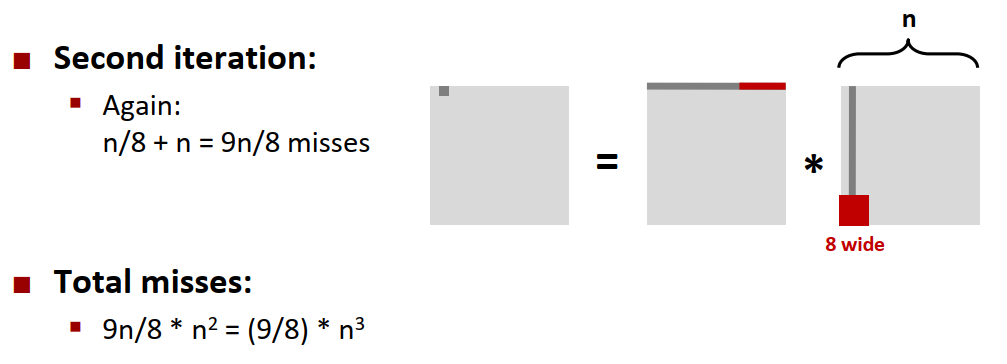
\includegraphics[width=0.8\textwidth]{memory/matrix-multiplication-unblocked-2.png}
\end{figure}
若采用分块策略:
\begin{figure}[H]
    \centering
    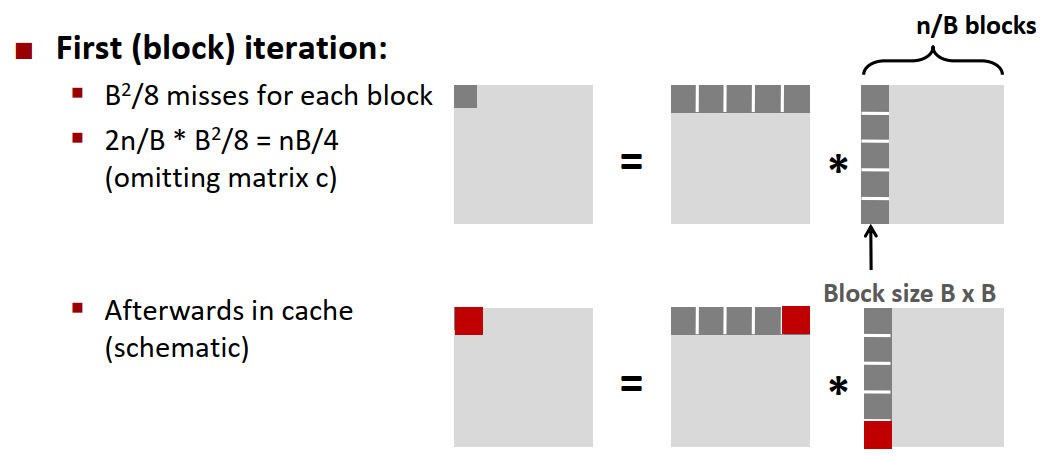
\includegraphics[width=0.8\textwidth]{memory/matrix-multiplication-blocked-1.png}
\end{figure}
\begin{figure}[H]
    \centering
    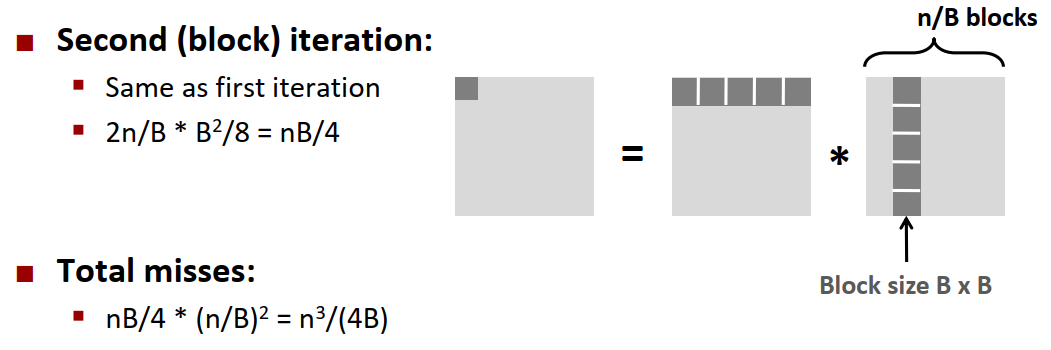
\includegraphics[width=0.8\textwidth]{memory/matrix-multiplication-blocked-2.png}
\end{figure}

比较发现,块大小 B 越大,未命中次数越少,但要求 $3B^2 < C$。

\newpage